% !TeX program = pdflatex
% !TeX encoding = UTF-8
% !TeX spellcheck = en_US
%%
%%%%%%%%%%%%%%%%%%%%%%%%%%%%%%%%%%%%%%%%%%%%%%%%%%%%%%%%%%%%%%%%%%%%%%%%%%%%%%%%
%%
%% A0 landscape poster for the Master's Thesis Seminar poster session.
%%
%% Title:      Dense Confidence and Inference-Time Scaling
%% Author:     Hannes Brantner
%% Institute:  Institute for Machine Learning, JKU Linz
%% Supervisor: Sepp Hochreiter (Co-Supervisors: Johannes Schimunek, Christoph Bartmann)
%%
%% The poster deliberately shares its substantive content with main-thesis.tex
%% rather than duplicating it:
%%   * csvmetrics.tex       -- every result number is the same live CSV lookup
%%                             used by the thesis result tables (single source).
%%   * acronyms.tex         -- the acronym definitions (loaded with [nolist] so
%%                             no List of Acronyms is typeset on the poster).
%%   * architecture_tikz.tex -- the training-time data-flow diagram, identical
%%                             to fig:architecture in the thesis.
%%
%% Build with the repository build script (pdflatex engine, the default):
%%   ./build.sh main-poster
%%
%%%%%%%%%%%%%%%%%%%%%%%%%%%%%%%%%%%%%%%%%%%%%%%%%%%%%%%%%%%%%%%%%%%%%%%%%%%%%%%%

\documentclass[17pt, a0paper, landscape, margin=12mm, innermargin=14mm,
	blockverticalspace=11mm, colspace=14mm, subcolspace=8mm]{tikzposter}

%% --- Fonts: clean sans-serif body to match a modern AI-lab poster ----------
\usepackage[T1]{fontenc}
\usepackage[utf8]{inputenc}
\renewcommand{\familydefault}{\sfdefault}

%% --- Math and tables --------------------------------------------------------
\usepackage{amsmath}
\usepackage{amssymb}
\usepackage{booktabs}
\usepackage{array}

%% --- TikZ libraries required by the shared architecture diagram -------------
\usepackage{tikz}
\usetikzlibrary{arrows.meta,positioning,shapes.geometric,calc,fit,backgrounds}

%% --- Acronyms: define them (shared file) but do not typeset a list ----------
\usepackage[nolist]{acronym}
%% On a poster, which is read non-linearly, the package's first-use expansion is
%% meaningless, so every \ac* variant simply prints the short (italic) form.
\DeclareRobustCommand{\acit}[1]{\textit{\acs{#1}}}
\DeclareRobustCommand{\acpit}[1]{\textit{\acsp{#1}}}
\DeclareRobustCommand{\acfit}[1]{\textit{\acs{#1}}}
\DeclareRobustCommand{\acfpit}[1]{\textit{\acsp{#1}}}
\DeclareRobustCommand{\aclf}[1]{\acl{#1}~(\acs{#1})}
\DeclareRobustCommand{\aclfp}[1]{\aclp{#1}~(\acsp{#1})}

%% --- Live result numbers, shared verbatim with the thesis result tables -----
%%%%%%%%%%%%%%%%%%%%%%%%%%%%%%%%%%%%%%%%%%%%%%%%%%%%%%%%%%%%%%%%%%%%%%%%%%%%%%%%
%% csvmetrics.tex
%%
%% Pure-LaTeX dynamic CSV value lookup for thesis result tables.
%% Backed by pgfplotstable: each CSV is read exactly once at load time
%% into a named table handle. Cells in the result tables then reference
%% scalars via \csvms{<handle>}{<metric_prefix>} or \csvv{<handle>}{<column>}.
%%
%% Paths are relative to the latexmk working directory, which is thesis/
%% (the build.sh Docker mount sets -w /work/thesis). CSV files therefore
%% live one level up under ../data/evaluation/final/.
%%%%%%%%%%%%%%%%%%%%%%%%%%%%%%%%%%%%%%%%%%%%%%%%%%%%%%%%%%%%%%%%%%%%%%%%%%%%%%%%

\usepackage{pgfplotstable}

%% ----------------------------------------------------------------------------
%% Helper macros
%% ----------------------------------------------------------------------------

%% \csvv{<table>}{<column>} -- print a single scalar value (formatted, 3 dec.)
\newcommand{\csvv}[2]{%
	\pgfplotstablegetelem{0}{\detokenize{#2}}\of{#1}%
	\pgfmathprintnumber[fixed,fixed zerofill,precision=3]{\pgfplotsretval}%
}

%% \csvms{<table>}{<metric_prefix>} -- print "$mean{\pm}std$".
%% metric_prefix MUST omit the trailing /mean or /std suffix.
\newcommand{\csvms}[2]{%
	$\csvv{#1}{#2/mean}{\pm}\csvv{#1}{#2/std}$%
}

%% \csvmsraw{<table>}{<metric_prefix>} -- like \csvms but without surrounding $...$ (use inside math).
\newcommand{\csvmsraw}[2]{%
	\csvv{#1}{#2/mean}{\pm}\csvv{#1}{#2/std}%
}

%% \AccAfterRaw / \AccBeforeRaw -- math-mode-safe (no inner $...$) variants of \AccAfter / \AccBefore.
\newcommand{\AccAfterRaw}[2]{\csvmsraw{#1}{eval_after_train/answer/accuracy/#2_t=1.0}}
\newcommand{\AccBeforeRaw}[2]{\csvmsraw{#1}{eval_before_train/answer/accuracy/#2_t=1.0}}

%% \csvval{<table>}{<column>}{<precision>} -- single value at chosen precision.
\newcommand{\csvval}[3]{%
	\pgfplotstablegetelem{0}{\detokenize{#2}}\of{#1}%
	\pgfmathprintnumber[fixed,fixed zerofill,precision=#3]{\pgfplotsretval}%
}

%% \csvpct{<table>}{<column>}{<precision>} -- value as percentage (x100) followed by "\,\%".
\newcommand{\csvpct}[3]{%
	\pgfplotstablegetelem{0}{\detokenize{#2}}\of{#1}%
	\begingroup
	\pgfkeys{/pgf/fpu=true}%
	\pgfmathparse{\pgfplotsretval*100}%
	\pgfmathprintnumber[fixed,fixed zerofill,precision=#3]{\pgfmathresult}\,\%%
	\endgroup
}

%% \csvdelta{<tableA>}{<tableB>}{<column>}{<precision>} -- signed (A-B) value.
\newcommand{\csvdelta}[4]{%
	\pgfplotstablegetelem{0}{\detokenize{#3}}\of{#1}\edef\csvAval{\pgfplotsretval}%
	\pgfplotstablegetelem{0}{\detokenize{#3}}\of{#2}\edef\csvBval{\pgfplotsretval}%
	\begingroup
	\pgfkeys{/pgf/fpu=true}%
	\pgfmathparse{\csvAval-\csvBval}%
	\pgfmathprintnumber[fixed,fixed zerofill,precision=#4,print sign]{\pgfmathresult}%
	\endgroup
}

%% \csvdeltapp{<tableA>}{<tableB>}{<column>}{<precision>} -- signed (A-B)*100 (pp).
\newcommand{\csvdeltapp}[4]{%
	\pgfplotstablegetelem{0}{\detokenize{#3}}\of{#1}\edef\csvAval{\pgfplotsretval}%
	\pgfplotstablegetelem{0}{\detokenize{#3}}\of{#2}\edef\csvBval{\pgfplotsretval}%
	\begingroup
	\pgfkeys{/pgf/fpu=true}%
	\pgfmathparse{(\csvAval-\csvBval)*100}%
	\pgfmathprintnumber[fixed,fixed zerofill,precision=#4,print sign]{\pgfmathresult}%
	\endgroup
}

%% \csvxdelta{<tableA>}{<colA>}{<tableB>}{<colB>}{<precision>} -- signed (A-B), columns may differ.
\newcommand{\csvxdelta}[5]{%
	\pgfplotstablegetelem{0}{\detokenize{#2}}\of{#1}\edef\csvAval{\pgfplotsretval}%
	\pgfplotstablegetelem{0}{\detokenize{#4}}\of{#3}\edef\csvBval{\pgfplotsretval}%
	\begingroup
	\pgfkeys{/pgf/fpu=true}%
	\pgfmathparse{\csvAval-\csvBval}%
	\pgfmathprintnumber[fixed,fixed zerofill,precision=#5,print sign]{\pgfmathresult}%
	\endgroup
}

%% \csvxdeltapp{<tableA>}{<colA>}{<tableB>}{<colB>}{<precision>} -- signed (A-B)*100 (pp).
\newcommand{\csvxdeltapp}[5]{%
	\pgfplotstablegetelem{0}{\detokenize{#2}}\of{#1}\edef\csvAval{\pgfplotsretval}%
	\pgfplotstablegetelem{0}{\detokenize{#4}}\of{#3}\edef\csvBval{\pgfplotsretval}%
	\begingroup
	\pgfkeys{/pgf/fpu=true}%
	\pgfmathparse{(\csvAval-\csvBval)*100}%
	\pgfmathprintnumber[fixed,fixed zerofill,precision=#5,print sign]{\pgfmathresult}%
	\endgroup
}

%% \csvrelpct{<tableA>}{<tableB>}{<column>}{<precision>} -- (A-B)/B*100, the relative
%% improvement of A over B on a shared column. Unsigned magnitude is printed.
\newcommand{\csvrelpct}[4]{%
	\pgfplotstablegetelem{0}{\detokenize{#3}}\of{#1}\edef\csvAval{\pgfplotsretval}%
	\pgfplotstablegetelem{0}{\detokenize{#3}}\of{#2}\edef\csvBval{\pgfplotsretval}%
	\begingroup
	\pgfkeys{/pgf/fpu=true}%
	\pgfmathparse{(\csvAval-\csvBval)/\csvBval*100}%
	\pgfmathprintnumber[fixed,fixed zerofill,precision=#4]{\pgfmathresult}%
	\endgroup
}

%% \csvxrelpct{<tableA>}{<colA>}{<tableB>}{<colB>}{<precision>} -- (A-B)/B*100 across columns.
\newcommand{\csvxrelpct}[5]{%
	\pgfplotstablegetelem{0}{\detokenize{#2}}\of{#1}\edef\csvAval{\pgfplotsretval}%
	\pgfplotstablegetelem{0}{\detokenize{#4}}\of{#3}\edef\csvBval{\pgfplotsretval}%
	\begingroup
	\pgfkeys{/pgf/fpu=true}%
	\pgfmathparse{(\csvAval-\csvBval)/\csvBval*100}%
	\pgfmathprintnumber[fixed,fixed zerofill,precision=#5]{\pgfmathresult}%
	\endgroup
}

%% \csvxabsdelta{<tableA>}{<colA>}{<tableB>}{<colB>}{<precision>} -- |A-B| across columns.
\newcommand{\csvxabsdelta}[5]{%
	\pgfplotstablegetelem{0}{\detokenize{#2}}\of{#1}\edef\csvAval{\pgfplotsretval}%
	\pgfplotstablegetelem{0}{\detokenize{#4}}\of{#3}\edef\csvBval{\pgfplotsretval}%
	\begingroup
	\pgfkeys{/pgf/fpu=true}%
	\pgfmathparse{abs(\csvAval-\csvBval)}%
	\pgfmathprintnumber[fixed,fixed zerofill,precision=#5]{\pgfmathresult}%
	\endgroup
}

%% \csvabsdelta{<tableA>}{<tableB>}{<column>}{<precision>} -- |A-B| on a shared column.
\newcommand{\csvabsdelta}[4]{\csvxabsdelta{#1}{#3}{#2}{#3}{#4}}

%% \csvxabsdeltapp{<tableA>}{<colA>}{<tableB>}{<colB>}{<precision>} -- |A-B|*100 (pp).
\newcommand{\csvxabsdeltapp}[5]{%
	\pgfplotstablegetelem{0}{\detokenize{#2}}\of{#1}\edef\csvAval{\pgfplotsretval}%
	\pgfplotstablegetelem{0}{\detokenize{#4}}\of{#3}\edef\csvBval{\pgfplotsretval}%
	\begingroup
	\pgfkeys{/pgf/fpu=true}%
	\pgfmathparse{abs(\csvAval-\csvBval)*100}%
	\pgfmathprintnumber[fixed,fixed zerofill,precision=#5]{\pgfmathresult}%
	\endgroup
}

%% \csvabsdeltapp{<tableA>}{<tableB>}{<column>}{<precision>} -- |A-B|*100 on a shared column.
\newcommand{\csvabsdeltapp}[4]{\csvxabsdeltapp{#1}{#3}{#2}{#3}{#4}}

%% Pooled-standard-deviation helpers. Metric arguments omit the trailing /mean or /std.
%% The descriptive statistic is s_pool=sqrt((s_A^2+s_B^2)/2), and
%% d_pool=|mean_A-mean_B|/s_pool. These are not inferential pooled-variance estimates.
%% \csvxpoolstd{<tableA>}{<metricA>}{<tableB>}{<metricB>}{<precision>}
\newcommand{\csvxpoolstd}[5]{%
	\pgfplotstablegetelem{0}{\detokenize{#2/std}}\of{#1}\edef\csvAstd{\pgfplotsretval}%
	\pgfplotstablegetelem{0}{\detokenize{#4/std}}\of{#3}\edef\csvBstd{\pgfplotsretval}%
	\begingroup
	\pgfkeys{/pgf/fpu=true}%
	\pgfmathparse{sqrt((\csvAstd*\csvAstd+\csvBstd*\csvBstd)/2)}%
	\pgfmathprintnumber[fixed,fixed zerofill,precision=#5]{\pgfmathresult}%
	\endgroup
}

%% \csvpoolstd{<tableA>}{<tableB>}{<metric>}{<precision>} -- shared-metric pooled std.
\newcommand{\csvpoolstd}[4]{\csvxpoolstd{#1}{#3}{#2}{#3}{#4}}

%% \csvxpoolstdpp / \csvpoolstdpp -- pooled std multiplied by 100 (percentage points).
\newcommand{\csvxpoolstdpp}[5]{%
	\pgfplotstablegetelem{0}{\detokenize{#2/std}}\of{#1}\edef\csvAstd{\pgfplotsretval}%
	\pgfplotstablegetelem{0}{\detokenize{#4/std}}\of{#3}\edef\csvBstd{\pgfplotsretval}%
	\begingroup
	\pgfkeys{/pgf/fpu=true}%
	\pgfmathparse{sqrt((\csvAstd*\csvAstd+\csvBstd*\csvBstd)/2)*100}%
	\pgfmathprintnumber[fixed,fixed zerofill,precision=#5]{\pgfmathresult}%
	\endgroup
}
\newcommand{\csvpoolstdpp}[4]{\csvxpoolstdpp{#1}{#3}{#2}{#3}{#4}}

%% \csvxpoold{<tableA>}{<metricA>}{<tableB>}{<metricB>}{<precision>}
\newcommand{\csvxpoold}[5]{%
	\pgfplotstablegetelem{0}{\detokenize{#2/mean}}\of{#1}\edef\csvAmean{\pgfplotsretval}%
	\pgfplotstablegetelem{0}{\detokenize{#2/std}}\of{#1}\edef\csvAstd{\pgfplotsretval}%
	\pgfplotstablegetelem{0}{\detokenize{#4/mean}}\of{#3}\edef\csvBmean{\pgfplotsretval}%
	\pgfplotstablegetelem{0}{\detokenize{#4/std}}\of{#3}\edef\csvBstd{\pgfplotsretval}%
	\begingroup
	\pgfkeys{/pgf/fpu=true}%
	\pgfmathparse{abs(\csvAmean-\csvBmean)/sqrt((\csvAstd*\csvAstd+\csvBstd*\csvBstd)/2)}%
	\pgfmathprintnumber[fixed,fixed zerofill,precision=#5]{\pgfmathresult}%
	\endgroup
}

%% \csvpoold{<tableA>}{<tableB>}{<metric>}{<precision>} -- shared-metric d_pool.
\newcommand{\csvpoold}[4]{\csvxpoold{#1}{#3}{#2}{#3}{#4}}

%% Compact renderers that print both statistics. Use these inside math mode.
%% Native-scale form: s_pool=<...>, d_pool=<...>.
\newcommand{\csvxpoolstats}[6]{%
	s_{\mathrm{pool}}=\csvxpoolstd{#1}{#2}{#3}{#4}{#5},\,
	d_{\mathrm{pool}}=\csvxpoold{#1}{#2}{#3}{#4}{#6}%
}
\newcommand{\csvpoolstats}[5]{\csvxpoolstats{#1}{#3}{#2}{#3}{#4}{#5}}

%% Percentage-point form for answer accuracies: s_pool=<...> pp, d_pool=<...>.
\newcommand{\csvxpoolstatspp}[6]{%
	s_{\mathrm{pool}}=\csvxpoolstdpp{#1}{#2}{#3}{#4}{#5}\,\mathrm{pp},\,
	d_{\mathrm{pool}}=\csvxpoold{#1}{#2}{#3}{#4}{#6}%
}
\newcommand{\csvpoolstatspp}[5]{\csvxpoolstatspp{#1}{#3}{#2}{#3}{#4}{#5}}

%% \csvxratio{<tableA>}{<colA>}{<tableB>}{<colB>}{<precision>} -- A/B.
\newcommand{\csvxratio}[5]{%
	\pgfplotstablegetelem{0}{\detokenize{#2}}\of{#1}\edef\csvAval{\pgfplotsretval}%
	\pgfplotstablegetelem{0}{\detokenize{#4}}\of{#3}\edef\csvBval{\pgfplotsretval}%
	\begingroup
	\pgfkeys{/pgf/fpu=true}%
	\pgfmathparse{\csvAval/\csvBval}%
	\pgfmathprintnumber[fixed,fixed zerofill,precision=#5]{\pgfmathresult}%
	\endgroup
}
\newcommand{\csvratio}[4]{\csvxratio{#1}{#3}{#2}{#3}{#4}}

%% \csvsumabsdeltas{<tableA>}{<tableB>}{<reference>}{<column>}{<precision>}
%% prints |A-ref|+|B-ref|.
\newcommand{\csvsumabsdeltas}[5]{%
	\pgfplotstablegetelem{0}{\detokenize{#4}}\of{#1}\edef\csvAval{\pgfplotsretval}%
	\pgfplotstablegetelem{0}{\detokenize{#4}}\of{#2}\edef\csvBval{\pgfplotsretval}%
	\pgfplotstablegetelem{0}{\detokenize{#4}}\of{#3}\edef\csvRefval{\pgfplotsretval}%
	\begingroup
	\pgfkeys{/pgf/fpu=true}%
	\pgfmathparse{abs(\csvAval-\csvRefval)+abs(\csvBval-\csvRefval)}%
	\pgfmathprintnumber[fixed,fixed zerofill,precision=#5]{\pgfmathresult}%
	\endgroup
}

%% \csvcombinedeffectratio{<joint>}{<standaloneA>}{<standaloneB>}{<reference>}{<column>}{<precision>}
%% prints |joint-ref|/(|standaloneA-ref|+|standaloneB-ref|).
\newcommand{\csvcombinedeffectratio}[6]{%
	\pgfplotstablegetelem{0}{\detokenize{#5}}\of{#1}\edef\csvJointval{\pgfplotsretval}%
	\pgfplotstablegetelem{0}{\detokenize{#5}}\of{#2}\edef\csvAval{\pgfplotsretval}%
	\pgfplotstablegetelem{0}{\detokenize{#5}}\of{#3}\edef\csvBval{\pgfplotsretval}%
	\pgfplotstablegetelem{0}{\detokenize{#5}}\of{#4}\edef\csvRefval{\pgfplotsretval}%
	\begingroup
	\pgfkeys{/pgf/fpu=true}%
	\pgfmathparse{abs(\csvJointval-\csvRefval)/(abs(\csvAval-\csvRefval)+abs(\csvBval-\csvRefval))}%
	\pgfmathprintnumber[fixed,fixed zerofill,precision=#6]{\pgfmathresult}%
	\endgroup
}

%% \calcpct{<numerator>}{<denominator>}{<precision>} -- numerator/denominator*100 followed by %.
\newcommand{\calcpct}[3]{%
	\begingroup
	\pgfkeys{/pgf/fpu=true}%
	\pgfmathparse{#1/#2*100}%
	\pgfmathprintnumber[fixed,fixed zerofill,precision=#3]{\pgfmathresult}\,\%%
	\endgroup
}

%% Convenience wrappers for the recurring "eval_{after,before}_train/answer/accuracy/<rule>_t=1.0"
%% and "eval_{after,before}_train/confidence/<metric>" column families.
\newcommand{\AccAfter}[2]{\csvms{#1}{eval_after_train/answer/accuracy/#2_t=1.0}}
\newcommand{\AccBefore}[2]{\csvms{#1}{eval_before_train/answer/accuracy/#2_t=1.0}}
\newcommand{\ConfAfter}[2]{\csvv{#1}{eval_after_train/confidence/#2/mean}}
\newcommand{\ConfBefore}[2]{\csvv{#1}{eval_before_train/confidence/#2/mean}}

%% Percentage forms (value*100, with %).
\newcommand{\AccAfterPct}[3]{\csvpct{#1}{eval_after_train/answer/accuracy/#2_t=1.0/mean}{#3}}
\newcommand{\AccBeforePct}[3]{\csvpct{#1}{eval_before_train/answer/accuracy/#2_t=1.0/mean}{#3}}
\newcommand{\ConfAfterPct}[3]{\csvpct{#1}{eval_after_train/confidence/#2/mean}{#3}}
\newcommand{\ConfBeforePct}[3]{\csvpct{#1}{eval_before_train/confidence/#2/mean}{#3}}

%% Plain (non-percentage) single value at chosen precision.
\newcommand{\AccAfterV}[3]{\csvval{#1}{eval_after_train/answer/accuracy/#2_t=1.0/mean}{#3}}
\newcommand{\AccBeforeV}[3]{\csvval{#1}{eval_before_train/answer/accuracy/#2_t=1.0/mean}{#3}}
\newcommand{\ConfAfterV}[3]{\csvval{#1}{eval_after_train/confidence/#2/mean}{#3}}
\newcommand{\ConfBeforeV}[3]{\csvval{#1}{eval_before_train/confidence/#2/mean}{#3}}

%% Recurring derived-statistic wrappers for answer and confidence metric families.
%% Pool-stat arguments are: table A, table B, metric name, s_pool precision, d_pool precision.
\newcommand{\AccAfterPoolStats}[5]{%
	\csvpoolstatspp{#1}{#2}{eval_after_train/answer/accuracy/#3_t=1.0}{#4}{#5}%
}
\newcommand{\AccAfterXPoolStats}[6]{%
	\csvxpoolstatspp{#1}{eval_after_train/answer/accuracy/#2_t=1.0}{#3}{eval_after_train/answer/accuracy/#4_t=1.0}{#5}{#6}%
}
\newcommand{\ConfAfterPoolStats}[5]{%
	\csvpoolstats{#1}{#2}{eval_after_train/confidence/#3}{#4}{#5}%
}

%% Absolute post-training gaps on recurring metric families.
\newcommand{\AccAfterAbsDelta}[4]{%
	\csvabsdelta{#1}{#2}{eval_after_train/answer/accuracy/#3_t=1.0/mean}{#4}%
}
\newcommand{\AccAfterAbsDeltaPP}[4]{%
	\csvabsdeltapp{#1}{#2}{eval_after_train/answer/accuracy/#3_t=1.0/mean}{#4}%
}
\newcommand{\ConfAfterAbsDelta}[4]{%
	\csvabsdelta{#1}{#2}{eval_after_train/confidence/#3/mean}{#4}%
}

%% \AccAfterGapRange{<tableA>}{<tableB>}{<precision>} -- min--max absolute
%% percentage-point gap across Pass@1, Pass@4, MV, HC, and CW-MV.
\newcommand{\AccAfterGapRange}[3]{%
	\pgfplotstablegetelem{0}{\detokenize{eval_after_train/answer/accuracy/pass@1_t=1.0/mean}}\of{#1}\edef\csvApone{\pgfplotsretval}%
	\pgfplotstablegetelem{0}{\detokenize{eval_after_train/answer/accuracy/pass@1_t=1.0/mean}}\of{#2}\edef\csvBpone{\pgfplotsretval}%
	\pgfplotstablegetelem{0}{\detokenize{eval_after_train/answer/accuracy/pass@4_t=1.0/mean}}\of{#1}\edef\csvApfour{\pgfplotsretval}%
	\pgfplotstablegetelem{0}{\detokenize{eval_after_train/answer/accuracy/pass@4_t=1.0/mean}}\of{#2}\edef\csvBpfour{\pgfplotsretval}%
	\pgfplotstablegetelem{0}{\detokenize{eval_after_train/answer/accuracy/majority_voting_t=1.0/mean}}\of{#1}\edef\csvAmv{\pgfplotsretval}%
	\pgfplotstablegetelem{0}{\detokenize{eval_after_train/answer/accuracy/majority_voting_t=1.0/mean}}\of{#2}\edef\csvBmv{\pgfplotsretval}%
	\pgfplotstablegetelem{0}{\detokenize{eval_after_train/answer/accuracy/highest_confidence_t=1.0/mean}}\of{#1}\edef\csvAhc{\pgfplotsretval}%
	\pgfplotstablegetelem{0}{\detokenize{eval_after_train/answer/accuracy/highest_confidence_t=1.0/mean}}\of{#2}\edef\csvBhc{\pgfplotsretval}%
	\pgfplotstablegetelem{0}{\detokenize{eval_after_train/answer/accuracy/confidence_weighted_majority_voting_t=1.0/mean}}\of{#1}\edef\csvAcwmv{\pgfplotsretval}%
	\pgfplotstablegetelem{0}{\detokenize{eval_after_train/answer/accuracy/confidence_weighted_majority_voting_t=1.0/mean}}\of{#2}\edef\csvBcwmv{\pgfplotsretval}%
	\begingroup
	\pgfkeys{/pgf/fpu=true}%
	\pgfmathparse{min(abs(\csvApone-\csvBpone),abs(\csvApfour-\csvBpfour),abs(\csvAmv-\csvBmv),abs(\csvAhc-\csvBhc),abs(\csvAcwmv-\csvBcwmv))*100}%
	\pgfmathprintnumber[fixed,fixed zerofill,precision=#3]{\pgfmathresult}%
	\text{--}%
	\pgfmathparse{max(abs(\csvApone-\csvBpone),abs(\csvApfour-\csvBpfour),abs(\csvAmv-\csvBmv),abs(\csvAhc-\csvBhc),abs(\csvAcwmv-\csvBcwmv))*100}%
	\pgfmathprintnumber[fixed,fixed zerofill,precision=#3]{\pgfmathresult}%
	\endgroup
}

%% Confidence-token inclusion / truncation percentages (already-fractional CSV cells).
\newcommand{\InclPctAfter}[2]{\csvpct{#1}{eval_after_train/answer/confidence_token_inclusion_percentage_t=1.0/mean}{#2}}
\newcommand{\TruncPctAfter}[2]{\csvpct{#1}{eval_after_train/answer/truncation_percentage_t=1.0/mean}{#2}}

%% ----------------------------------------------------------------------------
%% Preloaded answer-metric tables (one handle per training-time variant)
%% ----------------------------------------------------------------------------
\pgfplotstableread[col sep=comma]{../data/evaluation/final/agg_eval_before_train_answer_metrics_base.csv}\AnsBase
\pgfplotstableread[col sep=comma]{../data/evaluation/final/agg_eval_after_train_answer_metrics_noconfloss_noconfrew.csv}\AnsGRPO
\pgfplotstableread[col sep=comma]{../data/evaluation/final/agg_eval_after_train_answer_metrics_dense_confloss_noconfrew.csv}\AnsDenseAux
\pgfplotstableread[col sep=comma]{../data/evaluation/final/agg_eval_after_train_answer_metrics_dense_confloss_confrew.csv}\AnsDenseSR
\pgfplotstableread[col sep=comma]{../data/evaluation/final/agg_eval_after_train_answer_metrics_laser_confloss_noconfrew.csv}\AnsLaserAux
\pgfplotstableread[col sep=comma]{../data/evaluation/final/agg_eval_after_train_answer_metrics_laser_confloss_confrew.csv}\AnsLaserSR

%% Inference-time overlays (all on top of Dense Self-Rewarding checkpoint).
\pgfplotstableread[col sep=comma]{../data/evaluation/final/agg_eval_after_train_answer_metrics_dense_confloss_confrew_tempmod_nofilter.csv}\AnsTempNoFil
\pgfplotstableread[col sep=comma]{../data/evaluation/final/agg_eval_after_train_answer_metrics_dense_confloss_confrew_invtempmod_nofilter.csv}\AnsInvNoFil
\pgfplotstableread[col sep=comma]{../data/evaluation/final/agg_eval_after_train_answer_metrics_dense_confloss_confrew_notempmod_filter.csv}\AnsNoTempFil
\pgfplotstableread[col sep=comma]{../data/evaluation/final/agg_eval_after_train_answer_metrics_dense_confloss_confrew_tempmod_filter.csv}\AnsTempFil
\pgfplotstableread[col sep=comma]{../data/evaluation/final/agg_eval_after_train_answer_metrics_dense_confloss_confrew_invtempmod_filter.csv}\AnsInvFil

%% ----------------------------------------------------------------------------
%% Preloaded binary-classification tables (one handle per variant)
%% ----------------------------------------------------------------------------
\pgfplotstableread[col sep=comma]{../data/evaluation/final/concat_eval_before_train_bc_metrics_base.csv}\ConfBase
\pgfplotstableread[col sep=comma]{../data/evaluation/final/concat_eval_after_train_bc_metrics_noconfloss_noconfrew.csv}\ConfGRPO
\pgfplotstableread[col sep=comma]{../data/evaluation/final/concat_eval_after_train_bc_metrics_dense_confloss_noconfrew.csv}\ConfDenseAux
\pgfplotstableread[col sep=comma]{../data/evaluation/final/concat_eval_after_train_bc_metrics_dense_confloss_confrew.csv}\ConfDenseSR
\pgfplotstableread[col sep=comma]{../data/evaluation/final/concat_eval_after_train_bc_metrics_laser_confloss_noconfrew.csv}\ConfLaserAux
\pgfplotstableread[col sep=comma]{../data/evaluation/final/concat_eval_after_train_bc_metrics_laser_confloss_confrew.csv}\ConfLaserSR

\pgfplotstableread[col sep=comma]{../data/evaluation/final/concat_eval_after_train_bc_metrics_dense_confloss_confrew_tempmod_nofilter.csv}\ConfTempNoFil
\pgfplotstableread[col sep=comma]{../data/evaluation/final/concat_eval_after_train_bc_metrics_dense_confloss_confrew_invtempmod_nofilter.csv}\ConfInvNoFil
\pgfplotstableread[col sep=comma]{../data/evaluation/final/concat_eval_after_train_bc_metrics_dense_confloss_confrew_notempmod_filter.csv}\ConfNoTempFil
\pgfplotstableread[col sep=comma]{../data/evaluation/final/concat_eval_after_train_bc_metrics_dense_confloss_confrew_tempmod_filter.csv}\ConfTempFil
\pgfplotstableread[col sep=comma]{../data/evaluation/final/concat_eval_after_train_bc_metrics_dense_confloss_confrew_invtempmod_filter.csv}\ConfInvFil


%%%%%%%%%%%%%%%%%%%%%%%%%%%%%%%%%%%%%%%%%%%%%%%%%%%%%%%%%%%%%%%%%%%%%%%%%%%%%%%%
%% Theme and JKU-inspired colour palette
%%%%%%%%%%%%%%%%%%%%%%%%%%%%%%%%%%%%%%%%%%%%%%%%%%%%%%%%%%%%%%%%%%%%%%%%%%%%%%%%
\usetheme{Default}

\definecolor{jkublue}{HTML}{0A2D5E}   % deep navy for title and block headers
\definecolor{jkuaccent}{HTML}{E1006E} % JKU magenta accent for highlights

\colorlet{backgroundcolor}{white}
\colorlet{framecolor}{jkublue}
\colorlet{titlefgcolor}{white}
\colorlet{titlebgcolor}{jkublue}
\colorlet{blocktitlebgcolor}{jkublue}
\colorlet{blocktitlefgcolor}{white}
\colorlet{blockbodybgcolor}{white}
\colorlet{blockbodyfgcolor}{black}
\colorlet{innerblocktitlebgcolor}{white}
\colorlet{innerblocktitlefgcolor}{jkublue}
\colorlet{notefgcolor}{white}
\colorlet{notebgcolor}{jkuaccent}
\colorlet{noteframecolor}{jkuaccent}

%% Rounded, generously padded cards for both blocks and the title bar.
\useblockstyle[titleinnersep=14pt, bodyinnersep=20pt, roundedcorners=20,
	linewidth=1pt, titleoffsety=2pt]{Default}

\definetitlestyle{jkutitle}{
	width=\textwidth, roundedcorners=24, linewidth=0pt, innersep=24pt,
	titletotopverticalspace=3mm, titletoblockverticalspace=11mm,
	titlegraphictotitledistance=10pt, titletextscale=1
}{
	\begin{scope}[line width=\titlelinewidth, rounded corners=\titleroundedcorners]
		\draw[color=titlebgcolor, fill=titlebgcolor]
		(\titleposleft,\titleposbottom) rectangle (\titleposright,\titlepostop);
	\end{scope}
}
\usetitlestyle{jkutitle}

%% Plain white background (no gradient / decorations).
\definebackgroundstyle{jkubackground}{
	\draw[line width=0pt, color=white, fill=white]
	(bottomleft) rectangle (topright);
}
\usebackgroundstyle{jkubackground}

%% Remove the "created with tikzposter" footer.
\tikzposterlatexaffectionproofoff

%% Highlighted headline statistic (intentionally large; the only oversized text).
\newcommand{\statbox}[2]{%
	\begin{minipage}[t]{0.18\linewidth}
		\centering
		{\color{jkuaccent}\bfseries\fontsize{42}{46}\selectfont #1}\\[4pt]
		{\normalsize #2}
	\end{minipage}%
}

%%%%%%%%%%%%%%%%%%%%%%%%%%%%%%%%%%%%%%%%%%%%%%%%%%%%%%%%%%%%%%%%%%%%%%%%%%%%%%%%
%% Title
%%%%%%%%%%%%%%%%%%%%%%%%%%%%%%%%%%%%%%%%%%%%%%%%%%%%%%%%%%%%%%%%%%%%%%%%%%%%%%%%
\title{\parbox{\linewidth}{\raggedright Dense Confidence \& Inference-Time Scaling:\\[2pt]
		Extending \textit{LaSeR} for Reliable \acit{LLM} Reasoning}}
\author{Hannes Brantner}
\institute{Institute for Machine Learning, Johannes Kepler University Linz}

\makeatletter
\settitle{
	\begin{minipage}[c]{0.82\linewidth}
		\raggedright
		{\color{titlefgcolor}\bfseries\fontsize{46}{52}\selectfont \@title\par}
		\vspace{10pt}
		{\color{titlefgcolor}\large \textbf{\@author} (K1614466) \quad\textbar\quad
			Supervisor: \textbf{Sepp Hochreiter} \quad\textbar\quad
			Assistant Supervisors: Johannes Schimunek, Christoph Bartmann \quad\textbar\quad
			\@institute\par}
	\end{minipage}\hfill
	\begin{minipage}[c]{0.16\linewidth}
		\centering
		
\includegraphics[width=0.46\linewidth]{logos/jku_en_white.pdf}
	\end{minipage}
}
\makeatother

%%%%%%%%%%%%%%%%%%%%%%%%%%%%%%%%%%%%%%%%%%%%%%%%%%%%%%%%%%%%%%%%%%%%%%%%%%%%%%%%
\begin{document}

%% Declare the shared acronyms (typesets nothing thanks to the [nolist] option).
%%%%%%%%%%%%%%%%%%%%%%%%%%%%%%%%%%%%%%%%%%%%%%%%%%%%%%%%%%%%%%%%%%%%%%%%%%%%%%%%
%% 
%% List of acronyms (based on the acronyms package)
%% 

\addchap{\acronymname}
\begin{acronym}
	\acro{LLM}{Large Language Model}
\end{acronym}

%% 
%%%%%%%%%%%%%%%%%%%%%%%%%%%%%%%%%%%%%%%%%%%%%%%%%%%%%%%%%%%%%%%%%%%%%%%%%%%%%%%%


\maketitle

%%%%%%%%%%%%%%%%%%%%%%%%%%%%%%%%%%%%%%%%%%%%%%%%%%%%%%%%%%%%%%%%%%%%%%%%%%%%%%%%
%% Full-width headline / take-away banner
%%%%%%%%%%%%%%%%%%%%%%%%%%%%%%%%%%%%%%%%%%%%%%%%%%%%%%%%%%%%%%%%%%%%%%%%%%%%%%%%
\block{}{%
	\vspace{2pt}
	A $0.5\,$B-parameter \acit{LLM} is trained, in \emph{one} joint pass on commodity hardware, to be both an
	effective reasoner \emph{and} a calibrated judge of its own correctness. \textbf{\textit{Dense Confidence}}
	reads a repurposed control token's logit at \emph{every} step, maps it through a bounded scaled sigmoid, and
	supervises it with a class-rebalanced \acit{BCE} auxiliary loss alongside \acit{GRPO} --- at \emph{no}
	answer-quality cost --- then reuses the same per-token signal as an inference-time controller.
	\vspace{14pt}

	\centering
	\statbox{$\AccBeforePct{\AnsBase}{pass@1}{0} \mathrel{\raisebox{0.15em}{$\rightarrow$}} \AccAfterPct{\AnsDenseSR}{pass@1}{0}$}{\textit{Pass}@1 (\textit{Base} $\to$ \textit{Dense})}\hfill
	\statbox{$\ConfAfter{\ConfDenseAux}{mcc}$}{confidence \acit{MCC} (up to)}\hfill
	\statbox{$\InclPctAfter{\AnsDenseSR}{0}$}{confidence-token leakage}\hfill
	\statbox{$\AccAfterPct{\AnsDenseAux}{confidence_weighted_majority_voting}{0}$}{\acit{CW-MV} answer selection}\hfill
	\statbox{$1.75\,\%$}{of parameters trained}
	\vspace{4pt}
}

%%%%%%%%%%%%%%%%%%%%%%%%%%%%%%%%%%%%%%%%%%%%%%%%%%%%%%%%%%%%%%%%%%%%%%%%%%%%%%%%
\begin{columns}

	%% ===================== COLUMN 1 : PROBLEM AND IDEA =====================
	\column{0.30}

	\block{Motivation: dense in value, sparse in time}{%
		\acit{RLVR} restores objectivity to the reward channel by replacing the learned \acit{RLHF} preference
		model with a deterministic verifier --- but it does \emph{not} restore density. The reward stays a single
		bit per trajectory:
		\begin{itemize}
			\item A binary terminal verdict must be back-propagated across \emph{hundreds} of tokens, leaving
			      credit assignment to the policy gradient and inviting \textit{Goodharting} of the reward proxy.
			\item Self-rewarding methods let the policy be its own critic, but the closest one, \textit{LaSeR},
			      emits a \emph{single} self-assessment at the sequence terminus (sparse-in-time) and uses an
			      \emph{unbounded} log-probability that can drive the confidence-token logit high enough to
			      contaminate the sampling distribution.
		\end{itemize}
		\textbf{Goal.} Learn a \emph{bounded, per-token} confidence signal that is calibrated against correctness
		and cheap enough to train jointly with the policy.
	}

	\block{Research Questions}{%
		\begin{description}
			\item[\textcolor{jkuaccent}{RQ1}] Can a \emph{trajectory-wide} (dense) confidence signal be learned
			      jointly with \acit{GRPO} without degrading reasoning accuracy?
			\item[\textcolor{jkuaccent}{RQ2}] Does a bounded, logit-based parameterization eliminate the
			      confidence-token sampling interference reported for \textit{LaSeR}?
			\item[\textcolor{jkuaccent}{RQ3}] Does blending the intrinsic reward into the advantage improve
			      binary classification of correctness over pure answer accuracy?
			\item[\textcolor{jkuaccent}{RQ4}] Can the signal be exploited at \emph{inference} time --- answer
			      selection, temperature modulation, \acit{SMC} resampling --- to trade compute for accuracy or
			      calibration?
		\end{description}
	}

	\block{Method: \textit{Dense Confidence} (ours)}{%
		The \textit{Qwen2.5} vocabulary contains an unused control token (\texttt{<|vision\_pad|>}). A forward hook
		on the \acit{LM} head reads its logit $\ell_t^{\mathrm{conf}}$ at \emph{every} step and maps it to a
		bounded confidence
		\[
			c_t = \sigma\!\left(\tfrac{\pi}{\sigma_{\mathrm{conf}}\sqrt{3}}\,(\ell_t^{\mathrm{conf}}-\mu_{\mathrm{conf}})\right) \in [0,1].
		\]
		A class-rebalanced \acit{BCE} loss broadcasts the binary outcome reward $r_i$ to every position and is
		\emph{added} to the \acit{GRPO} objective (it is not optimized by the policy gradient itself):
		\[
			L_{\mathrm{total}} = -\mathcal{J}_{\mathrm{GRPO}}(\theta) + \beta_{\mathrm{conf}}\,L_{\mathrm{conf}},\quad
			L_{\mathrm{conf},i} = -\tfrac{1}{T_i}\!\sum_{t=1}^{T_i}\!\big[r_i\log c_{i,t} + (1{-}r_i)\log(1{-}c_{i,t})\big].
		\]
		Optionally (\emph{self-rewarding}) the trajectory-mean confidence $\bar c_i$ is blended into the advantage:
		\[
			A_i^{\mathrm{blended}} = (1-\alpha_{\mathrm{blend}})\,A_{r_i} + \alpha_{\mathrm{blend}}\,A_{\bar c_i}.
		\]
		The bounded sigmoid \emph{saturates}, so inflating the logit yields no free advantage: the token is never
		sampled and \emph{no} post-\acit{EOS} forward pass is needed.

		\textbf{Token hijacking.} Recycling an untrained slot is convenient --- it has no established meaning to
		disturb, so its logit can be freely re-aligned to the confidence task; were no empty slot available,
		appending a single new vocabulary row would deliver the same dedicated channel at negligible cost.
	}

	\block{Inference-time scaling (reuses the trained head, no retraining)}{%
		Three controllers reuse the \textit{Dense} head at evaluation only:
		\begin{itemize}
			\item \textbf{Answer selection.} Aggregate the $G$ generations by \acit{MV}, \acit{HC} (highest mean
			      confidence) or \acit{CW-MV} (confidence-weighted \acit{MV}).
			\item \textbf{Temperature modulation.} The decode temperature is a linear function of the running-mean
			      confidence over the last $H$ steps (with an inversion ablation).
			\item \textbf{\acit{SMC} particle filtering.} The $G$ rollouts form a particle set; low-confidence
			      particles are resampled from high-confidence donors of the same group, with explicit
			      \texttt{DynamicCache} surgery on the \acit{KV} cache.
		\end{itemize}
		The latter two are \emph{structurally exclusive} to \textit{Dense}: they consume a per-token signal that the
		last-token \textit{LaSeR} parameterization cannot provide.
		\par\vspace{157pt}
	}

	%% ===================== COLUMN 2 : ARCHITECTURE =====================
	\column{0.40}

	\block{Training-time architecture}{%
		\begin{center}
			\resizebox{0.72\linewidth}{!}{%%%%%%%%%%%%%%%%%%%%%%%%%%%%%%%%%%%%%%%%%%%%%%%%%%%%%%%%%%%%%%%%%%%%%%%%%%%%%%%%
%% architecture_tikz.tex
%%
%% Shared TikZ body for the \textit{Dense Confidence} training-time data-flow
%% diagram. Included verbatim by both main-thesis.tex (as fig:architecture) and
%% main-poster.tex so that the single source of truth for the architecture
%% figure is not duplicated across the two documents. The caller is responsible
%% for the surrounding float/\resizebox and the caption.
%%
%% Requires the TikZ libraries arrows.meta, positioning, shapes.geometric, calc,
%% fit and backgrounds, plus the acronym definitions (for \acfit) to be loaded.
%%%%%%%%%%%%%%%%%%%%%%%%%%%%%%%%%%%%%%%%%%%%%%%%%%%%%%%%%%%%%%%%%%%%%%%%%%%%%%%%
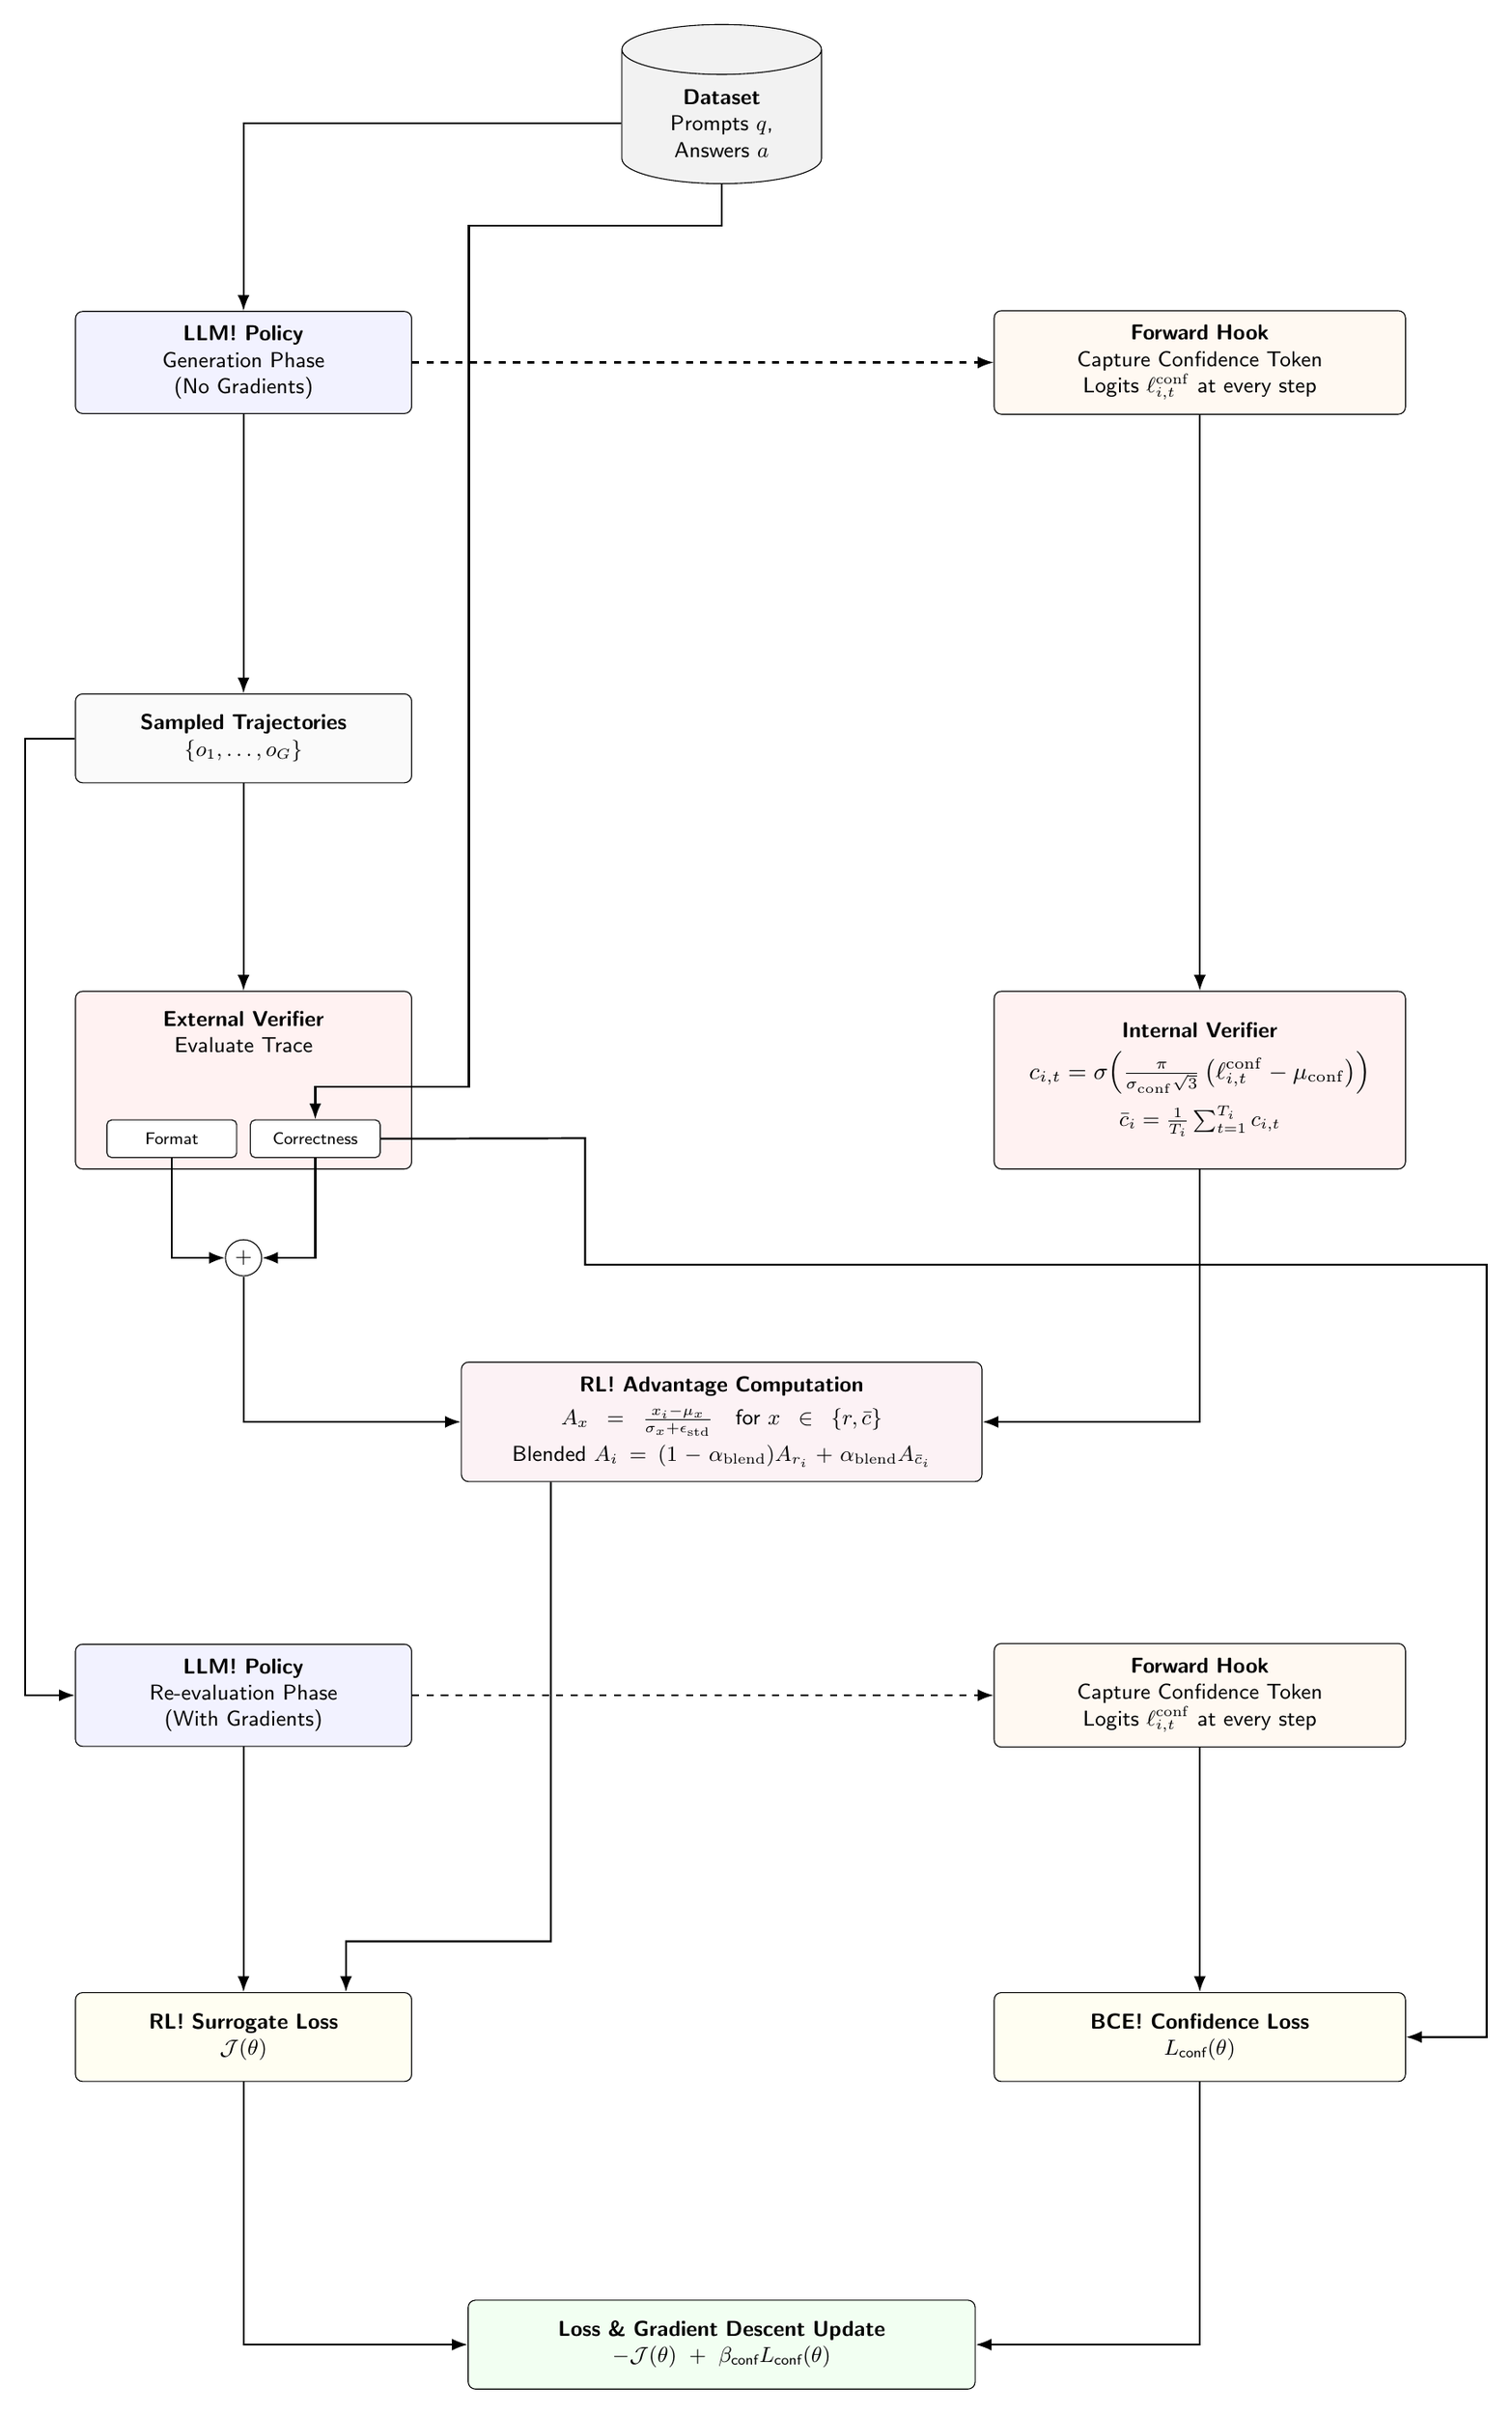
\begin{tikzpicture}[
		>=Latex,
		font=\small,
		box/.style={draw, rectangle, rounded corners=3pt, inner sep=6pt, align=center, fill=black!2, text width=4.5cm, minimum height=1.3cm},
		db/.style={draw, cylinder, cylinder uses custom fill, shape border rotate=90, aspect=0.25, inner sep=6pt, align=center, fill=black!5, text width=2.5cm, minimum height=1.5cm},
		arr/.style={thick, ->},
		dasharr/.style={thick, ->, dashed},
	]
	\node[db] (dataset) at (7, 3.5) {\textbf{Dataset}\\Prompts $q$, Answers $a$};
	\node[box, fill=blue!5] (policy1) at (0, 0) {\textbf{\acfit{LLM} Policy}\\Generation Phase\\(No Gradients)};
	\node[box] (traj) at (0, -5.5) {\textbf{Sampled Trajectories}\\$\{o_1, \dots, o_G\}$};
	\node[box, fill=red!5, minimum height=2.6cm, text width=4.5cm] (ext) at (0, -10.5) {};
	\node[align=center] at ($(ext.north) + (0, -0.6)$) {\textbf{External Verifier}\\Evaluate Trace};
	\node[draw, rectangle, fill=white, rounded corners=2pt, minimum height=0.55cm, minimum width=1.9cm, align=center] (form) at ($(ext.south) + (-1.05, 0.45)$) {\scriptsize Format};
	\node[draw, rectangle, fill=white, rounded corners=2pt, minimum height=0.55cm, minimum width=1.9cm, align=center] (corr) at ($(ext.south) + (1.05, 0.45)$) {\scriptsize Correctness};
	\node[draw, circle, inner sep=2pt, fill=white] (plus) at (0, -13.1) {$+$};
	\node[box, fill=orange!5, text width=5.6cm] (hook1) at (14, 0) {\textbf{Forward Hook}\\Capture Confidence Token\\Logits $\ell_{i,t}^{\mathrm{conf}}$ at every step};
	\node[box, fill=red!5, minimum height=2.6cm, text width=5.6cm] (int) at (14, -10.5) {};
	\node[align=center] at ($(int.north) + (0, -1.3)$) {\textbf{Internal Verifier}\\[5pt]\resizebox{5cm}{!}{$c_{i,t} = \sigma\!\left( \frac{\pi}{\sigma_{\mathrm{conf}}\sqrt{3}} \left(\ell_{i,t}^{\mathrm{conf}} - \mu_{\mathrm{conf}}\right) \right)$}\\[4pt]$\bar{c}_i = \frac{1}{T_i}\sum_{t=1}^{T_i} c_{i,t}$};
	\node[box, fill=purple!5, text width=7.2cm] (adv) at (7, -15.5) {\textbf{\acfit{RL} Advantage Computation}\\[3pt]$A_x = \frac{x_i - \mu_x}{\sigma_x + \epsilon_{\mathrm{std}}} \quad \text{for } x \in \{r, \bar{c}\}$\\[3pt]Blended $A_i = (1 - \alpha_{\mathrm{blend}}) A_{r_i} + \alpha_{\mathrm{blend}} A_{\bar{c}_i}$};
	\node[box, fill=blue!5, text width=4.5cm] (policy2) at (0, -19.5) {\textbf{\acfit{LLM} Policy}\\Re-evaluation Phase\\(With Gradients)};
	\node[box, fill=orange!5, text width=5.6cm] (hook2) at (14, -19.5) {\textbf{Forward Hook}\\Capture Confidence Token\\Logits $\ell_{i,t}^{\mathrm{conf}}$ at every step};
	\node[box, fill=yellow!5, text width=4.5cm] (loss_rl) at (0, -24.5) {\textbf{\acfit{RL} Surrogate Loss}\\$\mathcal{J}(\theta)$};
	\node[box, fill=yellow!5, text width=5.6cm] (loss_conf) at (14, -24.5) {\textbf{\acfit{BCE} Confidence Loss}\\$L_{\text{conf}}(\theta)$};
	\node[box, fill=green!5, text width=7.0cm] (update) at (7, -29.0) {\textbf{Loss \& Gradient Descent Update}\\$-\mathcal{J}(\theta) + \beta_{\text{conf}} L_{\text{conf}}(\theta)$};
	\draw[arr] (dataset.west) -| (policy1.north);
	\draw[arr] (policy1.south) -- (traj.north);
	\draw[dasharr] (policy1.east) -- (hook1.west);
	\draw[arr] (traj.south) -- (ext.north);
	\draw[arr] (hook1.south) -- (int.north);
	\draw[arr] (dataset.south) |- (3.3, 2.0) -- (3.3, -10.6) -| (corr.north);
	\draw[arr] (form.south) |- (plus.west);
	\draw[arr] (corr.south) |- (plus.east);
	\draw[arr] (plus.south) |- (adv.west);
	\draw[arr] (int.south) |- (adv.east);
	\draw[arr] (traj.west) -- (-3.2, -5.5) -- (-3.2, -19.5) -- (policy2.west);
	\draw[dasharr] (policy2.east) -- (hook2.west);
	\draw[arr] (policy2.south) -- (loss_rl.north);
	\draw[arr] ([xshift=-2.5cm]adv.south) |- (1.5, -23.1) -- ([xshift=1.5cm]loss_rl.north);
	\draw[arr] (corr.east) -- (5.0, -11.35) -- (5.0, -13.2) -- (18.2, -13.2) |- (loss_conf.east);
	\draw[arr] (hook2.south) -- (loss_conf.north);
	\draw[arr] (loss_rl.south) |- (update.west);
	\draw[arr] (loss_conf.south) |- (update.east);
\end{tikzpicture}
}
		\end{center}
		\vspace{4pt}
		The confidence-token logit is harvested \emph{twice} by the same \acit{LM}-head hook: gradient-free during
		generation (intrinsic reward) and with gradients during re-evaluation (auxiliary \acit{BCE} loss). The
		external verifier supplies the outcome bit $r$; the internal verifier maps each logit to $c_{i,t}\in[0,1]$.
	}

	\block{Selected references}{%
		[1] Yang et al. \textit{LaSeR: RL with Last-Token Self-Rewarding}, 2025.\quad
		[2] Shao et al. \textit{DeepSeekMath} (\acit{GRPO}), 2024.\quad
		[3] Cobbe et al. \textit{Training Verifiers to Solve Math Word Problems} (\acit{GSM8K}), 2021.\quad
		[4] Hu et al. \textit{LoRA}, 2021.\quad
		[5] Qwen Team. \textit{Qwen2.5 Technical Report}, 2025.\quad
		[6] Lew et al. \textit{\acit{SMC} Steering of LLMs}, 2023.
		\par\vspace{47pt}
	}

	%% ===================== COLUMN 3 : EVIDENCE AND CONCLUSION =====================
	\column{0.30}

	\block{Experimental setup}{%
		Filtered \aclf{GSM8K} ($N_{\mathrm{eval}}=1{,}222$, $G=4$/prompt) with a \texttt{Qwen2.5-0.5B-Instruct}
		policy. \acit{LoRA} plus the single confidence-token row train $\approx 1.75\,\%$ of the parameters;
		\acit{GRPO} with $\beta_{\mathrm{KL}}=0$. One epoch on a single \textit{NVIDIA GV100} (\texttt{float32}).
		Every row is the mean over \textbf{three} seeds ($\pm$ std). Six training variants: $\pm\ell$ (auxiliary
		loss), $\pm r$ (intrinsic reward); \textit{Dense} vs.\ \textit{LaSeR}.
	}

	\block{Results: training-time}{%
		\centering
		\setlength{\tabcolsep}{10pt}\renewcommand{\arraystretch}{1.15}
		\begin{tabular}{lcccc}
			\toprule
			\textbf{Variant}           & \textit{Pass}@1                       & \acit{MV}                                      & \acit{CW-MV}                                                                & \acit{MCC}                              \\
			\midrule
			\textit{Base}              & \AccBeforePct{\AnsBase}{pass@1}{0}    & \AccBeforePct{\AnsBase}{majority_voting}{0}    & ---                                                                         & ---                                     \\
			\acit{GRPO} ($-\ell-r$)    & \AccAfterPct{\AnsGRPO}{pass@1}{0}     & \AccAfterPct{\AnsGRPO}{majority_voting}{0}     & ---                                                                         & ---                                     \\
			\midrule
			\textit{Dense} ($+\ell-r$) & \AccAfterPct{\AnsDenseAux}{pass@1}{0} & \AccAfterPct{\AnsDenseAux}{majority_voting}{0} & \textbf{\AccAfterPct{\AnsDenseAux}{confidence_weighted_majority_voting}{0}} & \textbf{\ConfAfter{\ConfDenseAux}{mcc}} \\
			\textit{Dense} ($+\ell+r$) & \AccAfterPct{\AnsDenseSR}{pass@1}{0}  & \AccAfterPct{\AnsDenseSR}{majority_voting}{0}  & \AccAfterPct{\AnsDenseSR}{confidence_weighted_majority_voting}{0}           & \ConfAfter{\ConfDenseSR}{mcc}           \\
			\acit{LaSeR} ($+\ell-r$)   & \AccAfterPct{\AnsLaserAux}{pass@1}{0} & \AccAfterPct{\AnsLaserAux}{majority_voting}{0} & \AccAfterPct{\AnsLaserAux}{confidence_weighted_majority_voting}{0}          & \ConfAfter{\ConfLaserAux}{mcc}          \\
			\acit{LaSeR} ($+\ell+r$)   & \AccAfterPct{\AnsLaserSR}{pass@1}{0}  & \AccAfterPct{\AnsLaserSR}{majority_voting}{0}  & \AccAfterPct{\AnsLaserSR}{confidence_weighted_majority_voting}{0}           & \ConfAfter{\ConfLaserSR}{mcc}           \\
			\bottomrule
		\end{tabular}

		\raggedright\vspace{10pt}
		\textbf{Interpretation.}
		\begin{itemize}
			\item \textbf{No accuracy tax (RQ1).} \textit{Dense} matches \acit{GRPO} on \textit{Pass}@1, exceeds it on
			      \textit{Pass}@4; the head reaches \acit{MCC} up to $\ConfAfter{\ConfDenseAux}{mcc}$, \acit{ROC-AUC}
			      $>0.84$, while the untrained \acit{GRPO} control is random.
			\item \textbf{No leakage (RQ2).} The confidence token is sampled $\InclPctAfter{\AnsDenseSR}{0}$ of the
			      time --- the bounded sigmoid keeps its logit far below the vocabulary, removing both \textit{LaSeR}
			      symptoms (in-trace leakage and the extra forward pass).
			\item \textbf{Dense $>$ \textit{LaSeR} (RQ3).} \textit{Dense} sits $2$--$3$ pp above \textit{LaSeR} on every
			      answer metric; the unbounded \textit{LaSeR} reward collapses calibration once blended into the
			      advantage (\acit{MCC} $\ConfAfter{\ConfLaserAux}{mcc}\!\to\!\ConfAfter{\ConfLaserSR}{mcc}$).
			\item \textbf{Inference-time trade-off (RQ4).} On the \emph{same} checkpoint, tempmod $+$ \acit{SMC}
			      filtering lifts \acit{MCC} to the table's best $\ConfAfter{\ConfTempFil}{mcc}$ (small \textit{Pass}@1
			      cost) for calibration, while \acit{CW-MV} and inverse tempmod maximize answer accuracy --- compute is
			      traded for accuracy \emph{or} calibration, no retraining.
		\end{itemize}
	}

	\block{The per-step signal is an early-warning indicator}{%
		\begin{center}
			\includegraphics[width=0.82\linewidth]{charts/confidence_evolution_chart.pdf}
		\end{center}
		\vspace{2pt}
		Per-token confidence on a \emph{correct} (higher mean) vs.\ \emph{incorrect} (lower mean) \acit{GSM8K}
		rollout: the trajectories diverge \emph{hundreds of tokens early}, an internally decodable signal of
		eventual success or failure.
	}

	\block{Conclusion \& outlook}{%
		One repurposed token, an \acit{LM}-head hook, and a class-rebalanced \acit{BCE} auxiliary yield a calibrated,
		per-token confidence head at $0.5\,$B parameters with \emph{no} answer-quality cost and \emph{no} extra
		forward pass. The same head decouples calibration from answer accuracy at inference time on one checkpoint.
		Gains should grow with scale, data, and particle budget $G$; the head is a natural \acit{PRM} distillation
		target. \textbf{Code:} \texttt{github.com/Oidlichtnwoada/rl\_for\_llms}
		\par\vspace{140pt}
	}

\end{columns}

\end{document}
